\section{Ejercicio 1}

\subsection{Parámetros de las compuertas lógicas}
En esta sección desarrollaremos sobre los parámetros esenciales de las compuertas lógicas y estos son los siguientes:

\subsubsection{Tensión de salida y entrada}
Cuando se realizan compuertas lógicas vamos a poder establecer un rango de tensión de entrada donde la compuerta va a reconocer como un 1 lógico y otra para el cual va a tomar como un 0. Para esos mismos rangos vamos a poder definir un rango de salida dada cuando se encuentra en estado alto y otro para cuando está en estado bajo.
Los parámetros van a llamarse:
\begin{itemize}
	\item $V_{IL}$: Tensión de entrada considerada un 1 lógico
	\item $V_{IH}$: Tensión de entrada considerada un 0 lógico
	\item $V_{OL}$: Tensión de salida considerando que envía un 0 lógico
	\item $V_{OH}$: Tensión de entrada considerando que envía un 1 lógico
\end{itemize}
La parte más importante de estos son:
\begin{itemize}
	\item $V_{IL_{max}}$
	\item $V_{IH_{min}}$
	\item $V_{OL_{max}}$
	\item $V_{OH_{min}}$
\end{itemize}
Estos son obtenidos al realizar el siguiente esquema:
\begin{figure}[H]
	\centering
	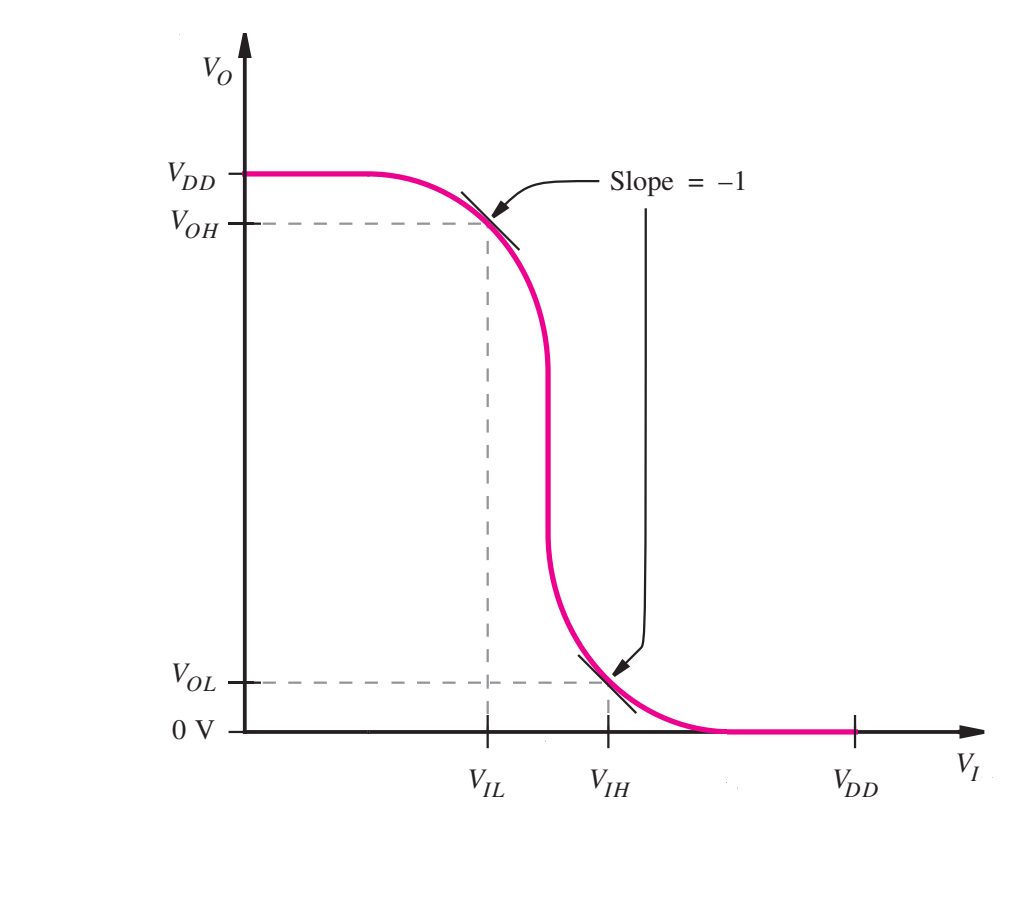
\includegraphics[width=0.4\textwidth]{Ejercicio1/Tensiones.png}
	\caption{High level y low level input y output}
\end{figure}

\subsubsection{Noise Margin}
Para determinar los márgenes de ruido se realizan las siguientes cuentas:
$$NM_{L}=|V_{OL}-V_{IL}|$$
$$NM_{H}=|V_{OH}-V_{IH}|$$

\subsubsection{Tiempo de propagación}
Son los tiempos en que tarda en cambiar la salida acorde a lo recibido en la entrada en otras palabras, es lo que tarda en cambiar la salida desde el momento en que recibió la entrada. Estos se miden como se va a visualizar a continuación:
\begin{figure}[H]
	\centering
	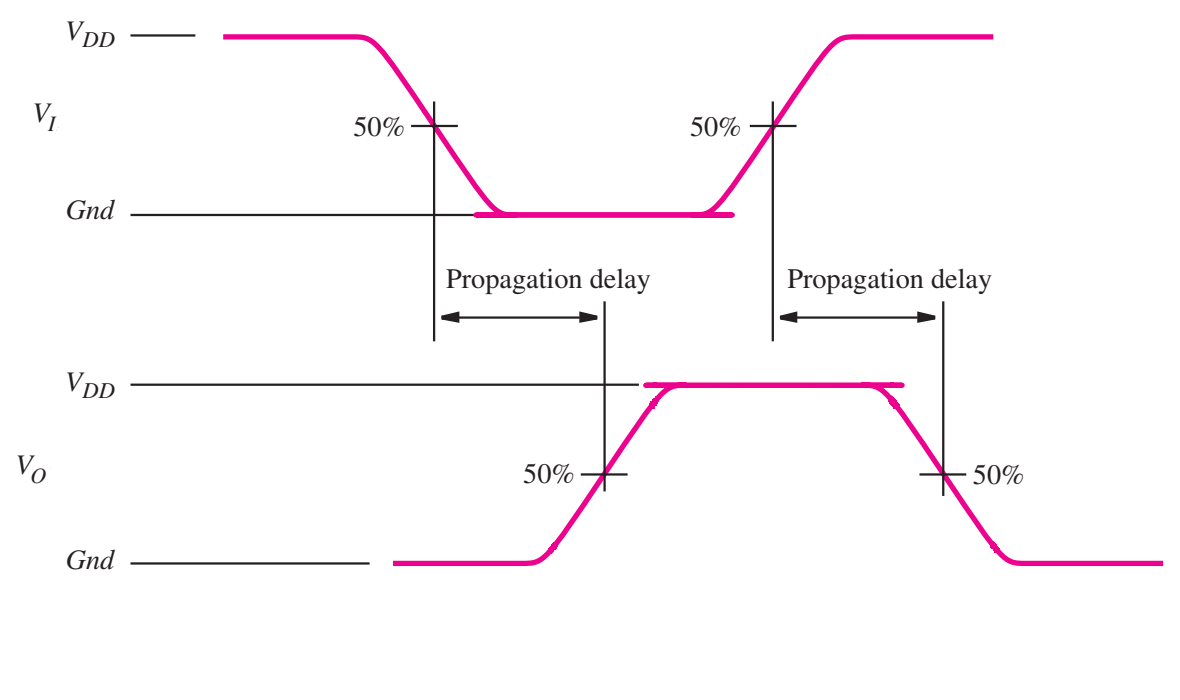
\includegraphics[width=0.3\textwidth]{Ejercicio1/Propagacion.png}
	\caption{Tiempos de propagación}
\end{figure}
Como se puede observar, hay dos tiempos de propagación, una de alto a bajo y el otro de bajo a alto.

\subsubsection{Tiempo de transición}
Es el Tiempo que le toma cambiar la salida de alta a bajo y viceversa, estas se definen como fall time y rise time. Se definen de la manera ilustrada en el gráfico:
\begin{figure}[H]
	\centering
	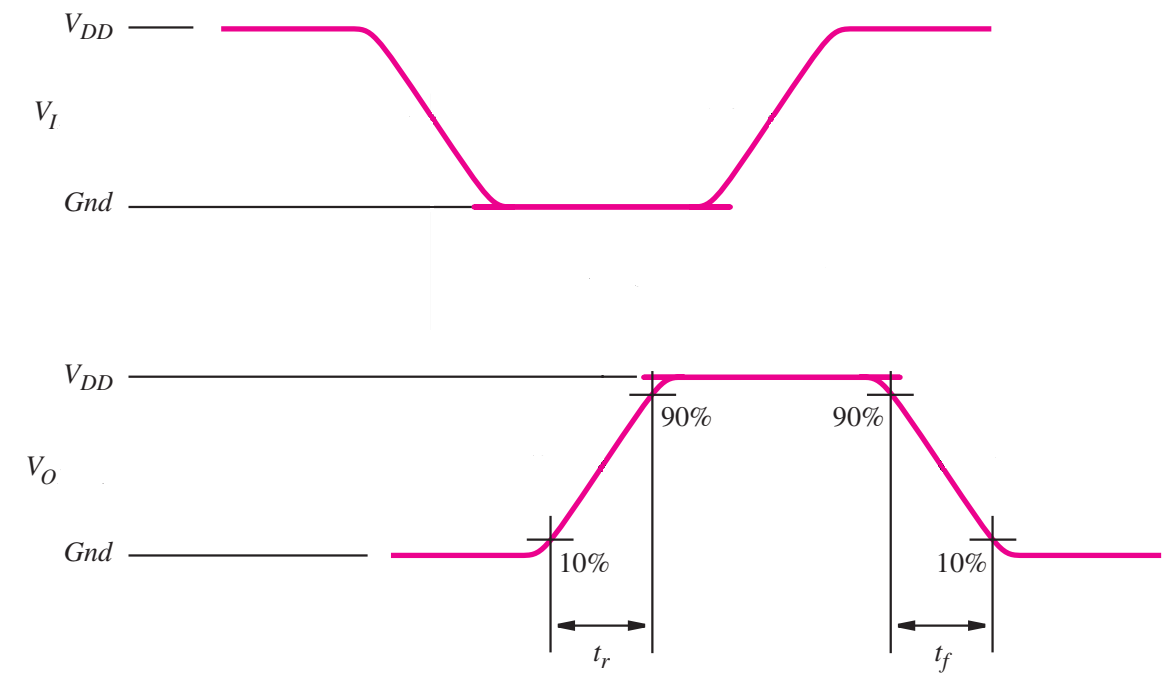
\includegraphics[width=0.3\textwidth]{Ejercicio1/Transicion.png}
	\caption{Tiempos de transición}
\end{figure}

\subsubsection{Corriente de salida}
Este parámetro es importante de definir dado que define el valor del fanout de la misma, dado que posea una carga solo capacitiva podemos definir la corriente como:
$$I=C\frac{dV_c}{dt}$$ 

\subsection{Tecnologías de las compuertas lógicas}
A continuación, hablaremos sobre los distintos tipos de tecnología así e ilustraremos los valores obtenidos de los parámetros de las arquitecturas aplicadas de cada tecnología. Estas son las siguientes:

\subsubsection{RTL}
La tecnología RTL consiste en conectar resistencias y transistores BJT para forma una compuerta lógica, donde la resistencia va a ser usado para polarizar el BJT. En la figura \ref{fig:eje1_1}, se encuentra la implementación de una compuerta NOT.
\begin{figure}[H]
	\centering
	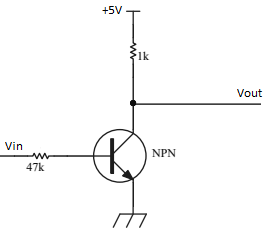
\includegraphics[width=0.2\textwidth]{Ejercicio1/RTL.png}
	\caption{NOT RTL}
	\label{fig:eje1_1}
\end{figure}
De la misma se obtuvieron los siguientes parámetros:
\begin{table}[H]
	\centering
	\begin{tabular}{|c|c|c|}
		\hline
		Parámetros & Valor sin carga & Valor con carga\\
		\hline
		$V_{IL_{max}}$ & 259 mV & 508 mV\\
		\hline
		$V_{IH_{min}}$ & 1.76 V & 1.72 V\\
		\hline
		$V_{OL_{max}}$ & 93 mV & 151 mV\\
		\hline
		$V_{OH_{min}}$ & 4.98 V & 4.98 V\\
		\hline
		$NM_{L}$ & 166 mV & 357 mV\\
		\hline
		$NM_{H}$ & 3.22 V & 3.26 V\\
		\hline
		Propagation delay High-to-Low & 371 nSeg &  548 nSeg\\
		\hline
		Propagation delay Low-to-High & 2.52 $\mu Seg$ &  3 $\mu Seg$\\
		\hline
		Fall time & 330 nSeg & 482 nSeg \\
		\hline
		Rise time & 1.07 $\mu Seg$ & 2.41 $\mu Seg$\\
		\hline
		Output current & 4.96 mA & 139 $\mu A$\\
		\hline
	\end{tabular}
\end{table}

\subsubsection{TTL}
La tecnología TTL consiste en conectar resistencias y transistores BJT para forma una compuerta lógica, donde vamos a polarizar el BJT que define la salida con otro BJT. En la figura \ref{fig:eje1_2}, se encuentra la implementación de una compuerta NOT.
\begin{figure}[H]
	\centering
	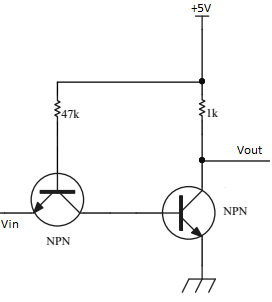
\includegraphics[width=0.2\textwidth]{Ejercicio1/TTL.png}
	\caption{NOT TTL}
	\label{fig:eje1_2}
\end{figure}
De la misma se obtuvieron los siguientes parámetros:
\begin{table}[H]
	\centering
	\begin{tabular}{|c|c|c|}
		\hline
		Parámetros & Valor sin carga & Valor con carga\\
		\hline
		$V_{IL_{max}}$ & 402 mV & 387 mV\\
		\hline
		$V_{IH_{min}}$ & 1.62 V & 1.62 V\\
		\hline
		$V_{OL_{max}}$ & 45 mV & 45 mV\\
		\hline
		$V_{OH_{min}}$ & 4.97 V & 4.97 V\\
		\hline
		$NM_{L}$ & 357 mV & 342 mV\\
		\hline
		$NM_{H}$ & 3.35 V & 3.35 V\\
		\hline
		Propagation delay High-to-Low & $<13$ nSeg & $<13$ nSeg\\
		\hline
		Propagation delay Low-to-High & 212 nSeg & 896 nSeg\\
		\hline
		Fall time & 52 nSeg & 184 nSeg\\
		\hline
		Rise time & 192 nSeg & 2.35 $\mu Seg$\\
		\hline
		Output current & 5 mA & 1.7 mA\\
		\hline
	\end{tabular}
\end{table}

\subsubsection{MOS}
La tecnología MOS consiste en conectar resistencias y transistores MOS para forma una compuerta lógica. En la figura \ref{fig:eje1_3}, se encuentra la implementación de una compuerta NOT.
\begin{figure}[H]
	\centering
	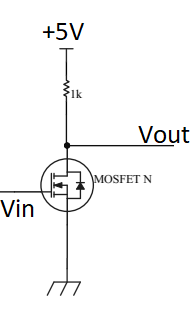
\includegraphics[width=0.2\textwidth]{Ejercicio1/MOS.png}
	\caption{NOT MOS}
	\label{fig:eje1_3}
\end{figure}
De la misma se obtuvieron los siguientes parámetros:
\begin{table}[H]
	\centering
	\begin{tabular}{|c|c|c|}
		\hline
		Parámetros & Valor sin carga & Valor con carga\\
		\hline
		$V_{IL_{max}}$ & 1.91 V & 1.98 V\\
		\hline
		$V_{IH_{min}}$ & 2.62 V & 2.64 V\\
		\hline
		$V_{OL_{max}}$ & 12 mV & 23 mV\\
		\hline
		$V_{OH_{min}}$ & 4.96 V & 4.94 V\\
		\hline
		$NM_{L}$ & 1.89 V & 1.78 V\\
		\hline
		$NM_{H}$ & 2.34 V & 2.3 V\\
		\hline
		Propagation delay High-to-Low & $<13$ nSeg & 19 nSeg\\
		\hline
		Propagation delay Low-to-High & 80 nSeg & 707 nSeg\\
		\hline
		Fall time & 12 nSeg & 21 nSeg\\
		\hline
		Rise time & 158 nSeg & 2.18 $\mu Seg$\\
		\hline
		Output current & 5mA & 523 $\mu A$\\
		\hline
	\end{tabular}
\end{table}

\subsubsection{Comparación entre tecnologías}
\begin{table}[H]
	\centering
	\begin{tabular}{|c|c|c|c|}
		\hline
		\diagbox{Parámetros}{Tecnologías} & RTL	& TTL & MOS\\
		\hline
		$V_{IL_{max}}$ & Aprox. 1.7 V & Aprox. 1.7 V & Aprox 2 V\\
		\hline
		$V_{IH_{min}}$ & Orden 100 mV & Aporx. 2 veces el RTL & Apox. 2.7 V\\
		\hline
		$V_{OH_{min}}$ & Casi Vcc & Casi Vcc &  Casi Vcc\\
		\hline
		$V_{OL_{max}}$ & Orden 100mV & Orden 10mV  & Orden mV\\
		\hline
		\multirow{2}{*}{Noise Margin} & Alto $NM_{H}$ & \multirow{2}{*}{Igual al RTL} & Menor $NM_{H}$ al resto\\
		 & bajo $NM_{L}$ &  & Medio $NM_{L}$\\
		\hline
		Propagation time & Orden $\mu Seg$ & Orden 100  nSeg & Orden 10 nSeg\\
		\hline
		Transition time & Orden $\mu Seg$ & Orden 100 nSeg & Orden de los nSeg\\
		\hline
		Output current & Orden 100 $\mu A$ & Orden mA & Alrededor 0.5 mA\\
		\hline
	\end{tabular}
\end{table}

Podemos concluir que dado que se quiera realizar un bajo consumo cuando uno se encuentre en estado bajo, es mejor utilizar compuertas MOS mientras que si se le da importancia a la cantidad de compuertas a conectarle atrás de está, es conveniente elegir TTL. Siempre que el problema de ruido no se encuentre considerablemente presente en bajo, las compuertas RTL y TTL son la mejor opción, pero si tenemos un presencia más uniforme de ruido tanto en estado bajo como en alta conviene la MOS. Por último, en cuanto a velocidad se destaca las MOS y en cuanto a niveles lógicos de entrada, la que requiere de menor tensión es la compuerta RTL.